\chapter{Results}\label{chapter_results}

This Chapter is concerned with the presentation of the results of a practical
application of the algorithms implemented in
Chapter~\ref{chapter_implementation} as well as and the performance of the
overall integrated system.

\section{Template Matching Tracker}
This Section presents with a qualitative analysis of both the adaptive and
non-adaptive Template Matching Trackers proposed in
Section~\ref{theoretical_framework_template_matching_trackers}. 

Both trackers were applied to the famous Hamburg taxi sequence \cite{} as an initial
test of their applicability to the Motion Tracking Problem.

The Template Trackers below were run for a threshold of 0.8.

\subsection{Simple Template Matching}\label{results_simple_template_matching}
The initial template used is the shown by the rectangular region around the car
in the first frame. The images shown correspond to almost equally spaced
samples of the 40 frame taxi sequence.

\begin{figure}\label{fig:simple_template_tracking}    
    \makebox[\linewidth][c]{
    \begin{tabular}{cccc}
        \subfloat{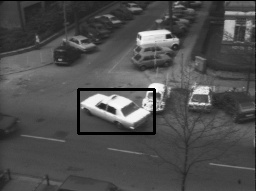
\includegraphics[width = 1.5in]{figures/results/simple_template_tracker/taxi_sequence/1.jpg}} &
        \subfloat{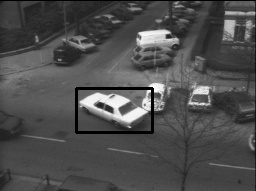
\includegraphics[width = 1.5in]{figures/results/simple_template_tracker/taxi_sequence/2.jpg}} &
        \subfloat{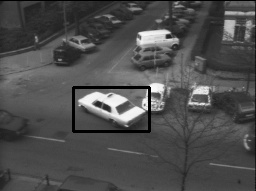
\includegraphics[width = 1.5in]{figures/results/simple_template_tracker/taxi_sequence/3.jpg}} &
        \subfloat{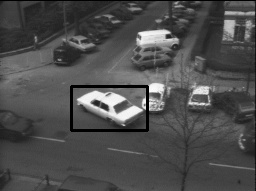
\includegraphics[width = 1.5in]{figures/results/simple_template_tracker/taxi_sequence/4.jpg}} \\

        \subfloat{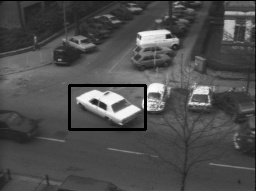
\includegraphics[width = 1.5in]{figures/results/simple_template_tracker/taxi_sequence/5.jpg}} &
        \subfloat{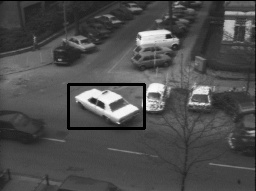
\includegraphics[width = 1.5in]{figures/results/simple_template_tracker/taxi_sequence/6.jpg}} &
        \subfloat{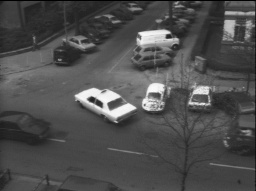
\includegraphics[width = 1.5in]{figures/results/simple_template_tracker/taxi_sequence/7.jpg}} &
        \subfloat{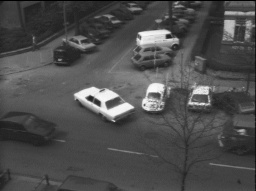
\includegraphics[width = 1.5in]{figures/results/simple_template_tracker/taxi_sequence/8.jpg}} \\
       
        \subfloat{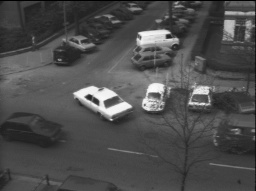
\includegraphics[width = 1.5in]{figures/results/simple_template_tracker/taxi_sequence/9.jpg}} &
        \subfloat{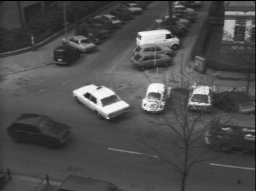
\includegraphics[width = 1.5in]{figures/results/simple_template_tracker/taxi_sequence/10.jpg}} &
        \subfloat{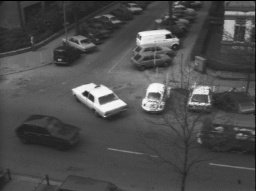
\includegraphics[width = 1.5in]{figures/results/simple_template_tracker/taxi_sequence/11.jpg}} &
        \subfloat{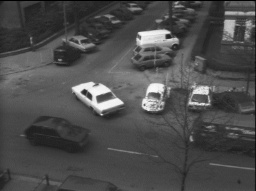
\includegraphics[width = 1.5in]{figures/results/simple_template_tracker/taxi_sequence/12.jpg}} \\
       
        \subfloat{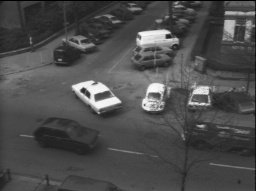
\includegraphics[width = 1.5in]{figures/results/simple_template_tracker/taxi_sequence/13.jpg}} &
        \subfloat{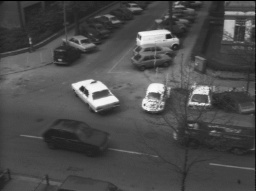
\includegraphics[width = 1.5in]{figures/results/simple_template_tracker/taxi_sequence/14.jpg}} &
        \subfloat{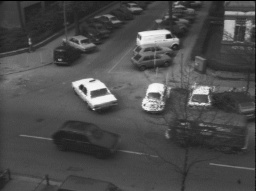
\includegraphics[width = 1.5in]{figures/results/simple_template_tracker/taxi_sequence/15.jpg}} &
        \subfloat{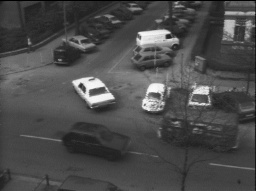
\includegraphics[width = 1.5in]{figures/results/simple_template_tracker/taxi_sequence/16.jpg}} \\   

        \end{tabular}}
    \caption{Simple Template Tracking Hamburg Sequence}
\end{figure}

In Figure~\ref{fig:simple_template_tracking} it can be seen that the Simple Template Matching Algorithm manages to track
the car up until frame 12 of the sequence, beyond which the rotation of the car
drives the Sum of Square Differences similarity measure between the initial template chosen in
$\mathbf{f}_0$ and the region of interest in $\mathbf{f}_{12}$ below the
threshold of 0.8.

Lowering the detection threshold allows the tracker to follow the
car for a larger amount of frames, however this is not a solution to the problem
as the tracker becomes more susceptible to noise, and is certainly not a good
model for robustness across different sequences.

An idea to get around the changing template, is the implementation of an
Adaptive Template Matching Algorithm.

\subsection{Adaptive Template Matching}\label{results_adaptive_template_matching}
As described in Section~\ref{theoretical_framework_adaptive_tm}, the assumption
that an object maintains the same appearance is only valid for an interval of
$K$ frames. Beyond this interval, $\mathbf{f}_{k}$ is sufficiently different
from $\mathbf{f}_{k+K}$ for our similarity measure to fall below the similarity
threshold, $\tau$.

The idea behind this variant of Template Tracker is that we update the
template which we are trying to match before the we traverse more than
$K$ frames.

The sequence in Figure~\ref{fig:adaptive_template_tracking} is generated by
updating the template every frame, the located object in frame,
$\mathbf{f}_{k-1}$. becomes the template for $\mathbf{f}_k$.

\begin{figure}     
    \makebox[\linewidth][c]{
    \begin{tabular}{cccc}
        \subfloat{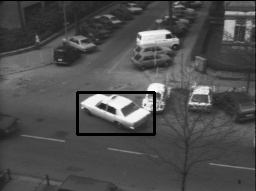
\includegraphics[width = 1.5in]{figures/results/adaptive_template_tracker/taxi_sequence/1.jpg}} &
        \subfloat{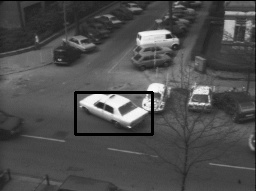
\includegraphics[width = 1.5in]{figures/results/adaptive_template_tracker/taxi_sequence/2.jpg}} &
        \subfloat{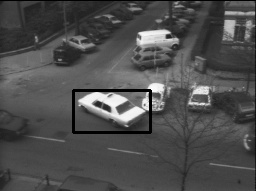
\includegraphics[width = 1.5in]{figures/results/adaptive_template_tracker/taxi_sequence/3.jpg}} &
        \subfloat{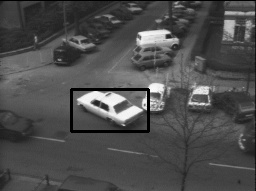
\includegraphics[width = 1.5in]{figures/results/adaptive_template_tracker/taxi_sequence/4.jpg}} \\

        \subfloat{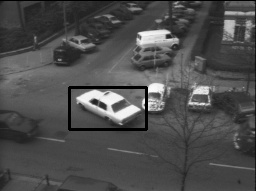
\includegraphics[width = 1.5in]{figures/results/adaptive_template_tracker/taxi_sequence/5.jpg}} &
        \subfloat{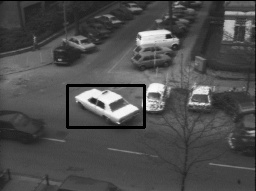
\includegraphics[width = 1.5in]{figures/results/adaptive_template_tracker/taxi_sequence/6.jpg}} &
        \subfloat{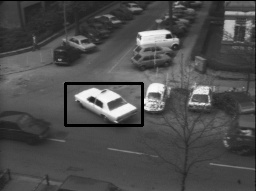
\includegraphics[width = 1.5in]{figures/results/adaptive_template_tracker/taxi_sequence/7.jpg}} &
        \subfloat{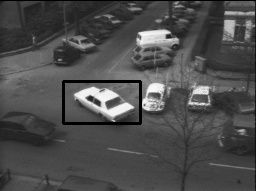
\includegraphics[width = 1.5in]{figures/results/adaptive_template_tracker/taxi_sequence/8.jpg}} \\
       
        \subfloat{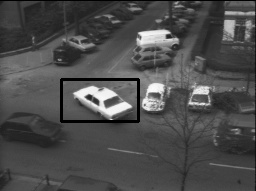
\includegraphics[width = 1.5in]{figures/results/adaptive_template_tracker/taxi_sequence/9.jpg}} &
        \subfloat{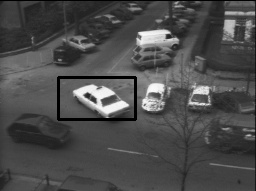
\includegraphics[width = 1.5in]{figures/results/adaptive_template_tracker/taxi_sequence/10.jpg}} &
        \subfloat{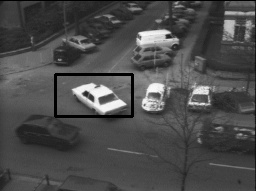
\includegraphics[width = 1.5in]{figures/results/adaptive_template_tracker/taxi_sequence/11.jpg}} &
        \subfloat{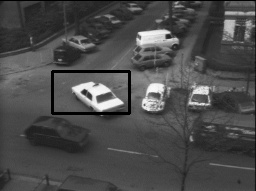
\includegraphics[width = 1.5in]{figures/results/adaptive_template_tracker/taxi_sequence/12.jpg}} \\
       
        \subfloat{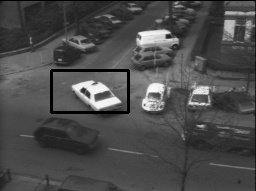
\includegraphics[width = 1.5in]{figures/results/adaptive_template_tracker/taxi_sequence/13.jpg}} &
        \subfloat{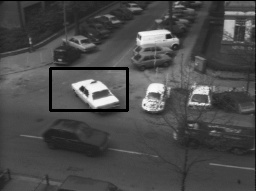
\includegraphics[width = 1.5in]{figures/results/adaptive_template_tracker/taxi_sequence/14.jpg}} &
        \subfloat{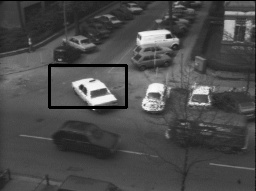
\includegraphics[width = 1.5in]{figures/results/adaptive_template_tracker/taxi_sequence/15.jpg}} &
        \subfloat{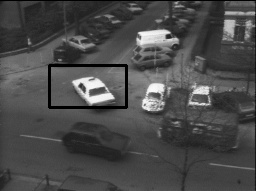
\includegraphics[width = 1.5in]{figures/results/adaptive_template_tracker/taxi_sequence/16.jpg}} \\   

        \end{tabular}}
    \caption{Adaptive Template Tracking Hamburg Sequence\label{fig:adaptive_template_tracking}}
\end{figure}

From Figure~\ref{fig:adaptive_template_tracking} it shows that the Adaptive
Template Tracker manages to locate the car within a bounding box in each frame
of the sequence. It should however be noted that there is a noticeable ``drift'' in
the localisation. 
This is due to the fact that the algorithm has no way of controlling the amount of
background noise that is allowed into the template.

\section{Colour Co-occurrence Histogram Detector}
This Section details the results of the CH-Detector implemented in
Section~\ref{implementation_ch}.

\subsection{Detection against Occlussion}
As discussed in Section~\ref{theoretical_framework_ch}, the rational behind
implementing the CH-Detector is assessing whether it could overcome the
shortcomings of the Template Matching approaches in terms of drift and lack of
generalisation.

The Adaptive Template Tracker failed immediately when faced with the challenge
of occlusion in the Girl sequence. We apply the CH-Detector to Occlusion on the
same challenge within sequence. To see whether it can successfully overcome the
challenge of occlusion.

In the experiment is performed as follows, We extract the model of the girl in
$\mathbf{f}_0$ of the sequence. We then proceed to use this model to localize
the frame in another frame, $\mathbf{f}_{138}$ was chose since it exhibits
occlusion of the model. 

The localization is performed by a two level hierarchical as described in
Section~\ref{implementation_ch}, with parameters $n_c=8$ and $n_d=12$ which
\cite{Change} rigorously proves to be the optimal values to minimize the False
Alarm Probability. (see Section~\ref{theoretical_framework_ch}).

Figure~\ref{fig:ch_partial_occlusion} details the results, the green bounding
box is the outcome of the initial coarse grained search of $\mathbf{f}_{139}$.
The result of the fine grained search within the green box region is highlighted
by the yellow bounding box. 
The CH-Detector effectively detects the girl within the $\mathbf{f}_{139}$ in
spite of significant occlusion on by the man obscuring the girl. 

\begin{figure}     
    \makebox[\linewidth][c]{
    \begin{tabular}{cc}
        \subfloat{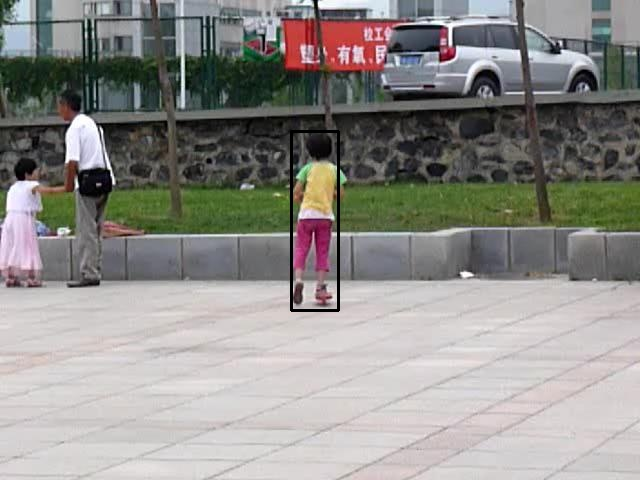
\includegraphics[width = 2.5in]{figures/results/ch_detector/results_girl/frame.jpg}} &
        \subfloat{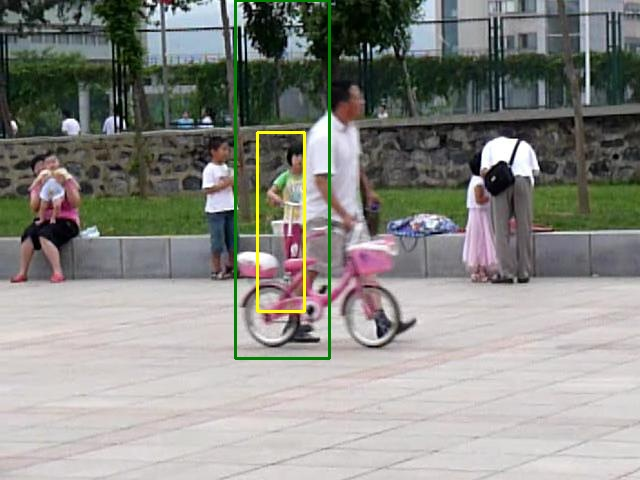
\includegraphics[width = 2.5in]{figures/results/ch_detector/results_girl/result.jpg}} \\

        \end{tabular}}
    \caption{Challenge: Partial Occlusion\label{fig:ch_partial_occlusion}
    }
\end{figure}


\section{Mean Shift Tracker}
This Section deals with the analysis of the Mean Shift Tracker (MST)
implemented in Section~\ref{implementation_mean_shift_tracker}. The analysis is
broken down into a set of experiments,

There are generally three parameters that a user can vary when using the mean
shift tracker. 
\begin{itemize}
    \item $\epsilon$ - step size bounding maximum mean shift vector magnitude
    \item $m$ - bin count of histograms
    \item $(h_x,h_y)$ - kernel dimensions and positioning around or on object
\end{itemize}
We subsequently assess the performance of the MST implementation
for varying parameters $\epsilon$ and $m$ for the sequence in order to see the
effect their on tracker performance, the goal being to select reasonable values
for the two parameters to asses the general practical performance of the Mean
Shift Tracker. 

We perform this assessment in a series of experiments, each of which is based on an image
sequence that exhibits one or more of the challenges to motion tracking outlined
in Section~\ref{literature_review_challenges}. 
 
The image sequences presented are taken from the datasets provided by the VOT2017
challenge \cite{VOT_TPAMI}.


\subsection{Effect of Step Size, $\epsilon$ on MST}\label{results_eps}


\subsection{Bin Count, $m$ on MST Execution time}\label{results_m}
This Experiment aims to quantitatively determine the effect of varying the
bin count, $m$ on the execution time of calculating the histogram, and computing
the Bhattacharyya coefficient.

The setup is simple enough, the execution time of the \textit{get\_pdf()} and
\textit{get\_BC()} functions was averaged over 1000 iterations for varying
values of m for a template of dimensions (100,100).

The effect of varying $m$ on histogram generation is shown in
Figure~\ref{fig:results_m_pdf}. There is not significant trend shown between the
bin count and the execution time of the get\_pdf() function. This makes sense
because we still iterate over all the pixels to allocate each of them to a
particular bin. The access time of the bins in the underlying numpy array is not
a significant bottle neck for array sizes (bin counts) ranging 1 to 256.

The effect of varying $m$ on the calculation of the Bhattacharyya coefficient is
detailed in Figure~\ref{fig:results_m_bc}. The execution time of the get\_BC() goes  

\Figure[width=0.7\columnwidth]{Graph showing effect of bin size (m) on execution time (ms) of \textit{get\_pdf()}}{results/mean_shift_tracker/results_m_pdf}

\Figure[width=0.7\columnwidth]{Graph showing effect of bin size (m) on execution time (ms) of \textit{get\_BC()}}{results/mean_shift_tracker/results_m_bc}

The Experiments 1-3 aim to assess performance of the MST in dealing with the
various motion tracking challenges, for varying sizes of Kernel initialisation.
The general idea is to compare the performance of a large kernel (Yellow)
encompassing the whole Object of Interest, and a smaller kernel (Green), that is
initialised around some feature of the larger object. 

For the subsequent experiments, the parameters $\epsilon$ and $m$ of the MST are
kept constant as $\epsilon=5$ and $m=8$. These choices were informed by the results in
Sections~\ref{results_eps} and~\ref{results_m}. 

\subsection{Experiment 1: Fish}
This sequence is one in which there are several fish, of which a distinctly yellow fish is
tracked. The challenges to motion tracking that arise in this image sequence are the following.
\begin{itemize}
    \item Occlusion (partial)
    \item Track Overlap
    \item Scaling 
    \item Ego motion (slight) 
\end{itemize}

The relevant sub-sequences of interest are documented below:

\subsubsection{Partial Occlusion}\label{mean_shift_partial_occlusion}
The relevant subsequence exhibiting Partial Occlusion is in from
$\mathbf{f}_{178}$ to $\mathbf{f}_{240}$ of the original sequence. This interval
is represented in Figure~\ref{fig:mean_shift_partial_occlusion}.

\begin{figure}     
    \makebox[\linewidth][c]{
    \begin{tabular}{cccc}
        \subfloat{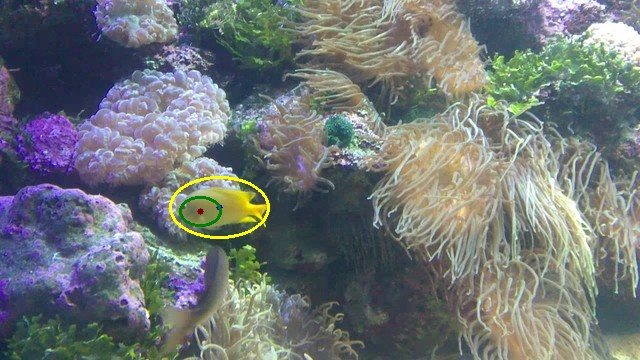
\includegraphics[width = 1.5in]{figures/results/mean_shift_tracker/fish3/occlusion/1.jpg}} &
        \subfloat{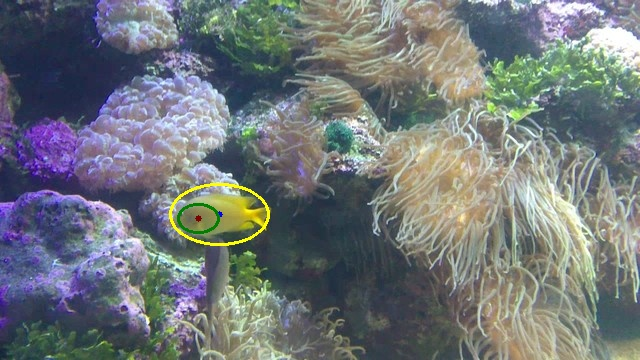
\includegraphics[width = 1.5in]{figures/results/mean_shift_tracker/fish3/occlusion/2.jpg}} &
        \subfloat{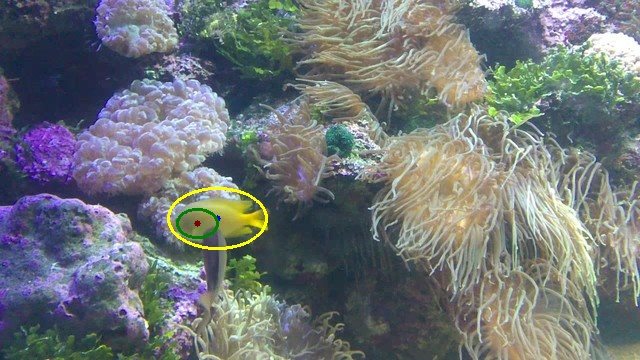
\includegraphics[width = 1.5in]{figures/results/mean_shift_tracker/fish3/occlusion/3.jpg}} &
        \subfloat{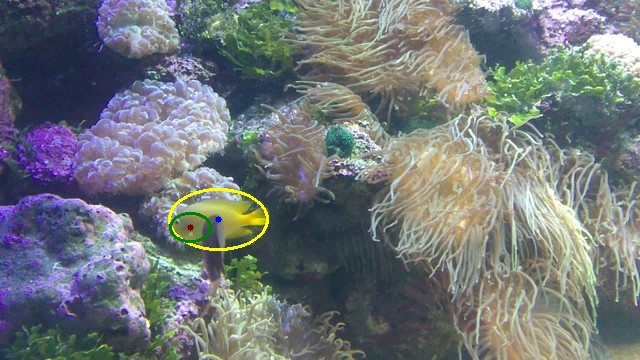
\includegraphics[width = 1.5in]{figures/results/mean_shift_tracker/fish3/occlusion/4.jpg}} \\

        \subfloat{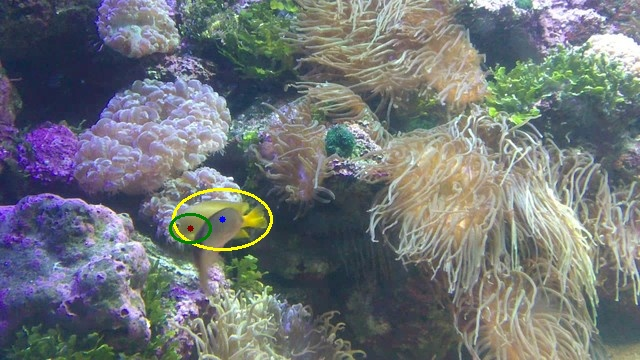
\includegraphics[width = 1.5in]{figures/results/mean_shift_tracker/fish3/occlusion/5.jpg}} &
        \subfloat{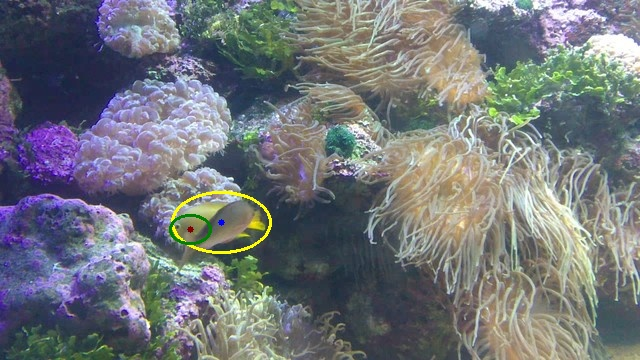
\includegraphics[width = 1.5in]{figures/results/mean_shift_tracker/fish3/occlusion/6.jpg}} &
        \subfloat{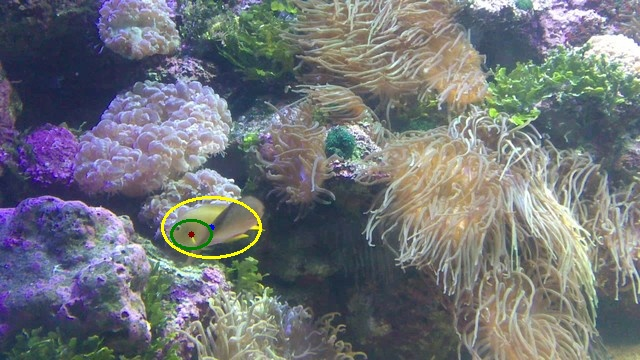
\includegraphics[width = 1.5in]{figures/results/mean_shift_tracker/fish3/occlusion/7.jpg}} &
        \subfloat{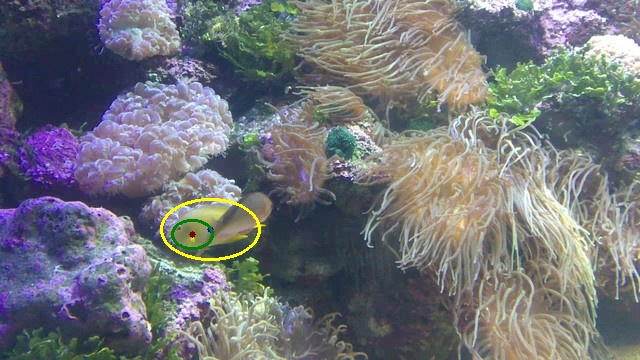
\includegraphics[width = 1.5in]{figures/results/mean_shift_tracker/fish3/occlusion/8.jpg}} \\
       
        \subfloat{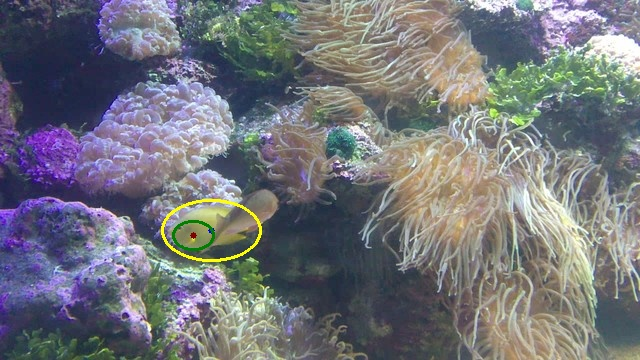
\includegraphics[width = 1.5in]{figures/results/mean_shift_tracker/fish3/occlusion/9.jpg}} &
        \subfloat{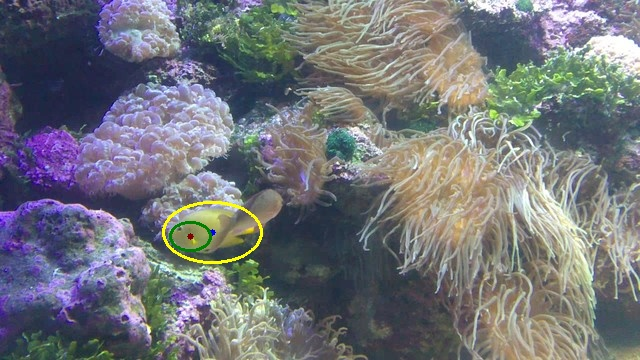
\includegraphics[width = 1.5in]{figures/results/mean_shift_tracker/fish3/occlusion/10.jpg}} &
        \subfloat{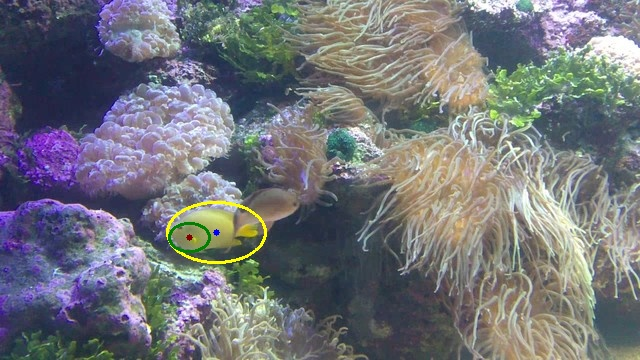
\includegraphics[width = 1.5in]{figures/results/mean_shift_tracker/fish3/occlusion/11.jpg}} &
        \subfloat{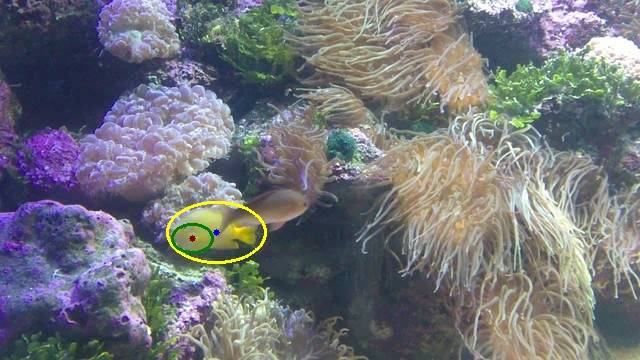
\includegraphics[width = 1.5in]{figures/results/mean_shift_tracker/fish3/occlusion/12.jpg}} \\
       
        \subfloat{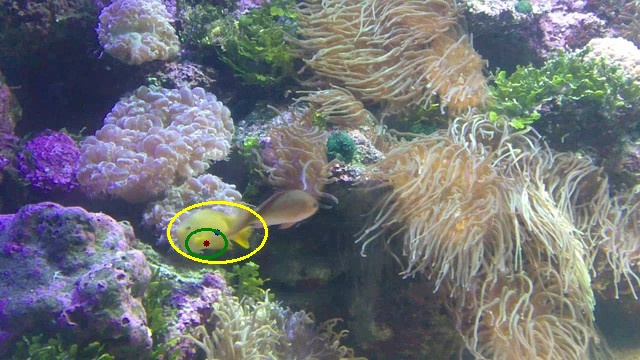
\includegraphics[width = 1.5in]{figures/results/mean_shift_tracker/fish3/occlusion/13.jpg}} &
        \subfloat{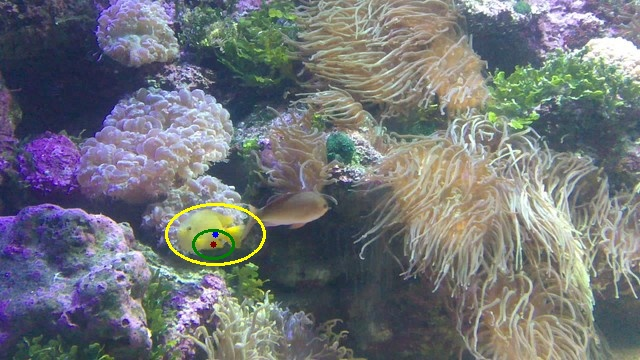
\includegraphics[width = 1.5in]{figures/results/mean_shift_tracker/fish3/occlusion/14.jpg}} &
        \subfloat{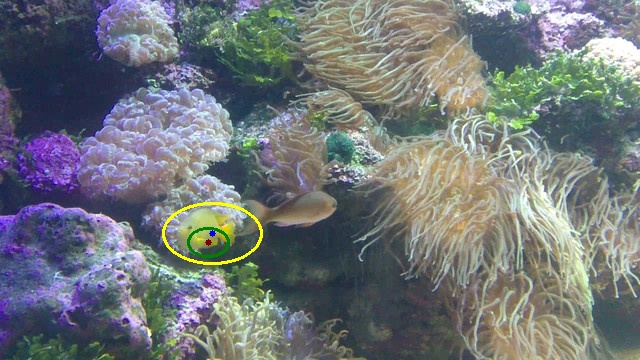
\includegraphics[width = 1.5in]{figures/results/mean_shift_tracker/fish3/occlusion/15.jpg}} &
        \subfloat{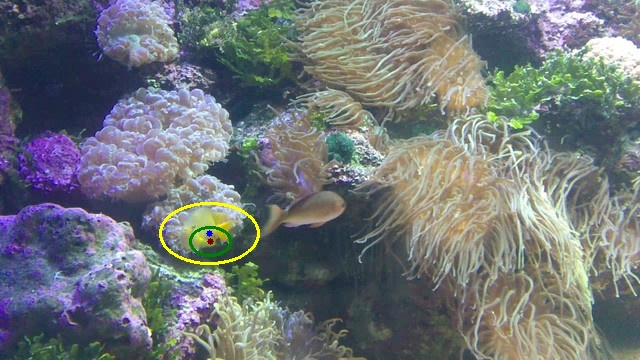
\includegraphics[width = 1.5in]{figures/results/mean_shift_tracker/fish3/occlusion/16.jpg}} \\   

        \end{tabular}}
    \caption{Challenge: Partial Occlusion\label{fig:mean_shift_partial_occlusion}
 }
\end{figure}

Our target, the yellow fish remains stationary from
$\mathbf{F_{1}}$ to $\mathbf{F_{16}}$. Both kernels are unaffected by the second
gray fish, occupying the same pixel space as our target. The tracker proves to be
robust to this form of occlusion and track overlap.
This is due to the fact that the target fish and the second fish are easily
distinguishable within the RGB colour-space from which we derive our histograms.
Therefore, the tracker is not drawn to the second fish.
As we still partially see a large part of our target when occluded, our
similarity, $\rho$ at the should remain greatest at the position of the target
despite the partial occlusion, which seems to be the case as the tracker does
not drift.

\subsubsection{Changing Orientation}

\begin{figure}     
    \makebox[\linewidth][c]{
    \begin{tabular}{cccc}
        \subfloat{\includegraphics[width = 1.5in]{figures/results/mean_shift_tracker/fish3/orientation/1.jpg}} &
        \subfloat{\includegraphics[width = 1.5in]{figures/results/mean_shift_tracker/fish3/orientation/2.jpg}} &
        \subfloat{\includegraphics[width = 1.5in]{figures/results/mean_shift_tracker/fish3/orientation/3.jpg}} &
        \subfloat{\includegraphics[width = 1.5in]{figures/results/mean_shift_tracker/fish3/orientation/4.jpg}} \\

        \subfloat{\includegraphics[width = 1.5in]{figures/results/mean_shift_tracker/fish3/orientation/5.jpg}} &
        \subfloat{\includegraphics[width = 1.5in]{figures/results/mean_shift_tracker/fish3/orientation/6.jpg}} &
        \subfloat{\includegraphics[width = 1.5in]{figures/results/mean_shift_tracker/fish3/orientation/7.jpg}} &
        \subfloat{\includegraphics[width = 1.5in]{figures/results/mean_shift_tracker/fish3/orientation/8.jpg}} \\
       
        \subfloat{\includegraphics[width = 1.5in]{figures/results/mean_shift_tracker/fish3/orientation/9.jpg}} &
        \subfloat{\includegraphics[width = 1.5in]{figures/results/mean_shift_tracker/fish3/orientation/10.jpg}} &
        \subfloat{\includegraphics[width = 1.5in]{figures/results/mean_shift_tracker/fish3/orientation/11.jpg}} &
        \subfloat{\includegraphics[width = 1.5in]{figures/results/mean_shift_tracker/fish3/orientation/12.jpg}} \\
       
        \subfloat{\includegraphics[width = 1.5in]{figures/results/mean_shift_tracker/fish3/orientation/13.jpg}} &
        \subfloat{\includegraphics[width = 1.5in]{figures/results/mean_shift_tracker/fish3/orientation/14.jpg}} &
        \subfloat{\includegraphics[width = 1.5in]{figures/results/mean_shift_tracker/fish3/orientation/15.jpg}} &
        \subfloat{\includegraphics[width = 1.5in]{figures/results/mean_shift_tracker/fish3/orientation/16.jpg}} \\   

        \end{tabular}}
    \caption{Challenge: Changing Orientation\label{fig:mean_shift_orientation}
 }
\end{figure}

\subsection{Experiment 2: Girl}
This sequence is one of a Girl in a park riding around on a scooter. She is
wearing a distinctive colourful outfit relative to the rest of the moving objects in the
scene, which consist mostly other humans.
The relevant challenges presented in this scene are:
\begin{itemize}
    \item Occlusion (complete)
    \item Scaling 
    \item Ego motion (slight) 
\end{itemize}

\subsubsection{Complete Occlusion}
The relevant subsequence exhibiting occlusion ranges from $\mathbf{f}_{97}$ to
$\mathbf{f}_{127}$ in the original sequence and is presented in Figure~\ref{fig:mean_shift_complete_occlusion}.

\begin{figure}    
    \makebox[\linewidth][c]{
    \begin{tabular}{cccc}
        \subfloat{\includegraphics[width = 1.5in]{figures/results/mean_shift_tracker/girl/occlusion/1.jpg}} &
        \subfloat{\includegraphics[width = 1.5in]{figures/results/mean_shift_tracker/girl/occlusion/2.jpg}} &
        \subfloat{\includegraphics[width = 1.5in]{figures/results/mean_shift_tracker/girl/occlusion/3.jpg}} &
        \subfloat{\includegraphics[width = 1.5in]{figures/results/mean_shift_tracker/girl/occlusion/4.jpg}} \\

        \subfloat{\includegraphics[width = 1.5in]{figures/results/mean_shift_tracker/girl/occlusion/5.jpg}} &
        \subfloat{\includegraphics[width = 1.5in]{figures/results/mean_shift_tracker/girl/occlusion/6.jpg}} &
        \subfloat{\includegraphics[width = 1.5in]{figures/results/mean_shift_tracker/girl/occlusion/7.jpg}} &
        \subfloat{\includegraphics[width = 1.5in]{figures/results/mean_shift_tracker/girl/occlusion/8.jpg}} \\
       
        \subfloat{\includegraphics[width = 1.5in]{figures/results/mean_shift_tracker/girl/occlusion/9.jpg}} &
        \subfloat{\includegraphics[width = 1.5in]{figures/results/mean_shift_tracker/girl/occlusion/10.jpg}} &
        \subfloat{\includegraphics[width = 1.5in]{figures/results/mean_shift_tracker/girl/occlusion/11.jpg}} &
        \subfloat{\includegraphics[width = 1.5in]{figures/results/mean_shift_tracker/girl/occlusion/12.jpg}} \\
       
        \subfloat{\includegraphics[width = 1.5in]{figures/results/mean_shift_tracker/girl/occlusion/13.jpg}} &
        \subfloat{\includegraphics[width = 1.5in]{figures/results/mean_shift_tracker/girl/occlusion/14.jpg}} &
        \subfloat{\includegraphics[width = 1.5in]{figures/results/mean_shift_tracker/girl/occlusion/15.jpg}} &
        \subfloat{\includegraphics[width = 1.5in]{figures/results/mean_shift_tracker/girl/occlusion/16.jpg}} \\   

        \end{tabular}
    }
    \caption{Challenge: Complete Occlusion\label{fig:mean_shift_complete_occlusion}}
\end{figure}

Figure~\ref{fig:mean_shift_complete_occlusion} shows the Mean Shift Tracker
managing to stay relocate the Girl after a man completely obscures her, we see
that the smaller Green Kernel is offset by man for a bit, whereby the larger
Yellow Kernel remains relatively stable.
The Green Kernel behaviour can be explained by the fact that it's model
$\hat(q)$ was defined solely around the Girl's yellow top. This is sufficiently
close for the Man's white top to cause a small drift which lasts only until the
girl is visible again upon which the.

\subsubsection{Scaling}

\begin{figure} 
    \makebox[\linewidth][c]{
    \begin{tabular}{cccc}
        \subfloat{\includegraphics[width = 1.5in]{figures/results/mean_shift_tracker/girl/scale/1.jpg}} &
        \subfloat{\includegraphics[width = 1.5in]{figures/results/mean_shift_tracker/girl/scale/2.jpg}} &
        \subfloat{\includegraphics[width = 1.5in]{figures/results/mean_shift_tracker/girl/scale/3.jpg}} &
        \subfloat{\includegraphics[width = 1.5in]{figures/results/mean_shift_tracker/girl/scale/4.jpg}} \\

        \subfloat{\includegraphics[width = 1.5in]{figures/results/mean_shift_tracker/girl/scale/5.jpg}} &
        \subfloat{\includegraphics[width = 1.5in]{figures/results/mean_shift_tracker/girl/scale/6.jpg}} &
        \subfloat{\includegraphics[width = 1.5in]{figures/results/mean_shift_tracker/girl/scale/7.jpg}} &
        \subfloat{\includegraphics[width = 1.5in]{figures/results/mean_shift_tracker/girl/scale/8.jpg}} \\
       
        \subfloat{\includegraphics[width = 1.5in]{figures/results/mean_shift_tracker/girl/scale/9.jpg}} &
        \subfloat{\includegraphics[width = 1.5in]{figures/results/mean_shift_tracker/girl/scale/10.jpg}} &
        \subfloat{\includegraphics[width = 1.5in]{figures/results/mean_shift_tracker/girl/scale/11.jpg}} &
        \subfloat{\includegraphics[width = 1.5in]{figures/results/mean_shift_tracker/girl/scale/12.jpg}} \\
       
        \subfloat{\includegraphics[width = 1.5in]{figures/results/mean_shift_tracker/girl/scale/13.jpg}} &
        \subfloat{\includegraphics[width = 1.5in]{figures/results/mean_shift_tracker/girl/scale/14.jpg}} &
        \subfloat{\includegraphics[width = 1.5in]{figures/results/mean_shift_tracker/girl/scale/15.jpg}} &
        \subfloat{\includegraphics[width = 1.5in]{figures/results/mean_shift_tracker/girl/scale/16.jpg}} \\   
    \end{tabular}}
    \caption{Challenge: Scale Change\label{fig:mean_shift_girl_scale}}
\end{figure}


\subsection{Experiment 3: Ants}
This image sequence is of multiple ants in motion within a Petri dish.

The challenges presented by this sequence are the following:
\begin{itemize}
    \item Target Speed
    \item Track Overlap
\end{itemize}

\subsubsection{Target Speed}\label{mean_shift_target_speed}
The relevant subsequence ranges from $\mathbf{f}_{202}$ to $\mathbf{f}_{250}$
in the original sequence.
In Figure~\ref{fig:mean_shift_target_speed}, $\mathbf{F}_{13}$ to $\mathbf{F}_{16}$
highlight this issue, as can be seen by the Green Kernel failing to track the
Ant for the due to its relatively large inter-frame displacement.

\begin{figure}
    \makebox[\linewidth][c]{
    \begin{tabular}{cccc}
        \subfloat{\includegraphics[width = 1.5in]{figures/results/mean_shift_tracker/ants/speed/1.jpg}} &
        \subfloat{\includegraphics[width = 1.5in]{figures/results/mean_shift_tracker/ants/speed/2.jpg}} &
        \subfloat{\includegraphics[width = 1.5in]{figures/results/mean_shift_tracker/ants/speed/3.jpg}} &
        \subfloat{\includegraphics[width = 1.5in]{figures/results/mean_shift_tracker/ants/speed/4.jpg}} \\

        \subfloat{\includegraphics[width = 1.5in]{figures/results/mean_shift_tracker/ants/speed/5.jpg}} &
        \subfloat{\includegraphics[width = 1.5in]{figures/results/mean_shift_tracker/ants/speed/6.jpg}} &
        \subfloat{\includegraphics[width = 1.5in]{figures/results/mean_shift_tracker/ants/speed/7.jpg}} &
        \subfloat{\includegraphics[width = 1.5in]{figures/results/mean_shift_tracker/ants/speed/8.jpg}} \\
       
        \subfloat{\includegraphics[width = 1.5in]{figures/results/mean_shift_tracker/ants/speed/9.jpg}} &
        \subfloat{\includegraphics[width = 1.5in]{figures/results/mean_shift_tracker/ants/speed/10.jpg}} &
        \subfloat{\includegraphics[width = 1.5in]{figures/results/mean_shift_tracker/ants/speed/11.jpg}} &
        \subfloat{\includegraphics[width = 1.5in]{figures/results/mean_shift_tracker/ants/speed/12.jpg}} \\
       
        \subfloat{\includegraphics[width = 1.5in]{figures/results/mean_shift_tracker/ants/speed/13.jpg}} &
        \subfloat{\includegraphics[width = 1.5in]{figures/results/mean_shift_tracker/ants/speed/14.jpg}} &
        \subfloat{\includegraphics[width = 1.5in]{figures/results/mean_shift_tracker/ants/speed/15.jpg}} &
        \subfloat{\includegraphics[width = 1.5in]{figures/results/mean_shift_tracker/ants/speed/16.jpg}} \\   
    \end{tabular}}
    \caption{Challenge: target speed losing small kernel\label{fig:mean_shift_ant_speed}}
\end{figure}

\begin{figure}
    \makebox[\linewidth][c]{
    \begin{tabular}{cccc}
        \subfloat{\includegraphics[width = 1.5in]{figures/results/mean_shift_tracker/ants/speed2/1.jpg}} &
        \subfloat{\includegraphics[width = 1.5in]{figures/results/mean_shift_tracker/ants/speed2/2.jpg}} &
        \subfloat{\includegraphics[width = 1.5in]{figures/results/mean_shift_tracker/ants/speed2/3.jpg}} &
        \subfloat{\includegraphics[width = 1.5in]{figures/results/mean_shift_tracker/ants/speed2/4.jpg}} \\
    \end{tabular}}
    \caption{Challenge: target speed losing large kernel\label{fig_mean_shift_ant_speed2}}
\end{figure}

Keeping in mind that a digital video is a sampling of an analogue scene.
In order to discuss the effect of the ``speed'' of a target on tracker
performance it is necessary to interpret this speed more clearly
as the magnitude of an object's inter-frame displacement, $\delta$ - which
we define as the distance between an object's
position between two adjacent frames $\mathbf{f}_k$ and $\mathbf{f}_{k+1}$.
This is an adequate formulation because, depending on the sampling frequency $f_s$ of
a particular sequence, a fast object such as a car sampled at a high $f_s$ can
have a smaller $\delta$ than a relatively slow snail sampled at a lower $f_s$. 

As the $\delta$ of an Object between $\mathbf{f}_k$ and $\mathbf{f}_{k+1}$ 
increases in magnitude, less of the Object lies within the dimensions
$(h_x,h_y)$ of the Kernel that we initialise at it's last known pixel location
$\mathbf{c_0}$ in $\mathbf{f}_k$. In terms of the mean shift tracking algorithm this simply
results in a larger mean shift vector, $\vec{m}$.

As shown in Experiment~\ref{results_varying_epsilon}, The Mean Shift Tracker's
parameter $\epsilon$ - which limits the allowed magnitude of $\vec{m}$ between
$\mathbf{f}_{k}$ and $\mathbf{f}_{k+1}$ - can increase the tracker's tolerance
to challenges such as Object speed and occlusion, at the
cost of increased track ``jitter''. 

However the Green Kernel throughout Figure~\ref{fig:mean_shift_ant_speed}
highlights the extreme case in which the kernel initialised at $\mathbf{c_0}$ in
$\mathbf{f}_{k+1}$ does not even partly contain the Target.  

We do see that the larger Yellow Kernel manages to track the Ant successfully
from $\mathbf{F_1}$ to $\mathbf{F_7}$ before changing tracks for a better closer
candidate as elaborated in section~\ref{mean_shift_track_overlap}.
Figure~\ref{fig:mean_shift_ant_speed2} shows $f_{271}$ to $f_{274}$ of the original
sequence, highlighting that even the larger Yellow Kernel can to track the if
at sufficiently high inter-frame displacement.

The results in Figures~\ref{mean_shift_ant_speed} tell us
that a larger kernel larger kernel size is more robust to the effects of large
$\delta$, but as Figure~\ref{fig:mean_shift_ant_speed2}, even a
kernel enclosing the whole object of interest can lose track of the object given
a sufficiently large $\delta$. It is also not feasible to increase our kernel
size largely beyond the object dimensions, as it would incorporate a lot of
noise into the object model $\hat(q)$, likely deteriorating tracker performance
when faced with other challenges.

It is important to note that a solution to the problem can be tied back to
sampling rate, $f_s$ used to obtain the sequence. If a higher sampling rate were
used, it would mean higher redundancy between frames with smaller $\delta$
values. An impractical solution therefore could be to try and obtain the
same sequence again, but sampled at a higher $f_s$.

This is likely unfeasible. Furthermore, one can imaging situations in which the
available technology is constrained by factors such as budget, size etc. In such
situations, we would still like to be able to track our object of interest.  A
possible solution could be to augment the basic Mean Shift Algorithm with other
forms of more information possibly from other tracking methodologies highlighted
in Figure\ref{fig:motion_tracking_taxonomy}. 

\subsubsection{Track Overlap}\label{mean_shift_track_overlap}
In Figure~\ref{fig:mean_shift_ant_speed}, $\mathbf{F}_5$ to $\mathbf{F}_{11}$
highlight this challenge. We have two ants coming within close proximity of
each other, we can see that the yellow kernel switches to track the second Ant
after the crossing of their tracks within the sequence. Let us refer to the
original ant as $A_0$ and the second ant as $A_1$. 

It is important at this point to highlight the differences between this case of
track overlap, and that detailed in Section~\ref{mean_shift_partial_occlusion},
in which, despite the tracks for the yellow fish and grey fish overlapping
entirely, the tracker remains remains unaffected.
The answer lies within the feature space our tracker is based on. Within the RGB colour space,
the yellow and grey fish are largely distinct. Hence the tracker will not be
drawn to the grey fish as it exits the Yellow Kernel.

In this case, the are two objects within the Yellow Kernel that are practically
indistinguishable within our chose feature space. One ant exits the Kernel, there exists
no gradient within the domain of the similarity function to draw the tracker away.

With $A_0$ and $A_1$ close to each other, The fact that $A_0$ moves with a high
velocity, means that the inter-frame displacement of $A_0$ between
$\mathbf{f}_k$ and $\mathbf{f}_{k+1}$ is easily be large enough to place $A_1$
closer to $A_0$ in $\mathbf{f}_{k+1}$, which makes the mean shift iteration
likely to pick $A_1$ as the target location in $\mathbf{f}_{k+1}$

\section{Graphical User Interface}
The implemented GUI System is shown below in Figure~\ref{fig:results_gui}

\Figure[width=1\columnwidth]{Image of the MOT System GUI implementation applying
the MS-Tracker to a fish sequence}{results/gui/first_look}

\subsection{I/O functionality}
The GUI allows a user to select and 

\subsection{Algorithm Integration}
The three algorithms discussed in Section~\ref{chapter_theoretical_framework}successfully integrated with the Front-end GUI. Their usage
within the GUI is shown in the subsequence sections.

\subsubsection{Template Trackers}

\subsubsection{Co-occurrence histogram Detector}

\subsubsection{Mean Shift Tracker}

\subsection{Parameter Selection}
In addition to implementing the algorithms, the parameters for the individual
algorithms can be varied by by the user.


\subsection{}
